\documentclass[portrait,a0paper]{baposter}

\usepackage{calc}
\usepackage{url}
\usepackage{amsmath}
\usepackage{amssymb}
\usepackage{relsize}
\usepackage{multirow}
\usepackage{booktabs}
\usepackage{graphicx}
\usepackage{multicol}
\usepackage[T1]{fontenc}
\usepackage{ae}
\usepackage{mathrsfs}
\usepackage{ifpdf}
\usepackage{wallpaper}

\renewcommand{\familydefault}{\sfdefault}

\ifpdf
	\pdfcompresslevel=9
	\pdfinfo
	{
		/Author (Luis Sanabria-Russo, Jaume Barcel\'{o}, Boris Bellalta)
		/Title (Fairness in Collision-Free WLANs)
		/Subject (Poster for INFOCOM 2013)
	}
\fi

\selectcolormodel{cmyk}

\definecolor{imdeanavy}{cmyk}{1,0.342,0,0.714}
%\definecolor{imdeabluedark}{cmyk}{0.628,0.345,0,0.431}
\definecolor{imdeabluedark}{cmyk}{0.23,0.11,0,0.33}
\definecolor{imdeabluelight}{cmyk}{0.372,0.208,0,0.114}
\definecolor{imdeacyan}{cmyk}{0.091,0.050,0,0.055}

\newenvironment{packeditemize}{
\begin{itemize}
	\setlength{\itemsep}{1pt}
	\setlength{\parskip}{0pt}
	\setlength{\parsep}{0pt}
}{\end{itemize}}

\begin{document}

\background
{
\begin{tikzpicture}[remember picture,overlay]%
\draw (current page.north west)+(-3.9pt,3.5pt) node[anchor=north west]
{
		\ifpdf
			
\includegraphics[width=\paperwidth+0.7pt]{background2-eps-converted-to.pdf}\\
		\else
			
\includegraphics[width=\paperwidth+0.7pt]{background2.eps}\\
		\fi
};
\end{tikzpicture}%
}

\begin{poster}
% Settings
{
	grid=no,
	columns=2,
	colspacing=1em,
	eyecatcher=no,
	borderColor=imdeanavy,
	textborder=rectangle,
  	titleColor=white,
    	authorColor=white,
	headerfont=\textsf,
	headerborder=closed,
	headershape=rectangle,
	headerColorOne=imdeabluedark,
	headerColorTwo=imdeabluedark,
	headerFontColor=white,
	boxColorOne=white,
	boxColorTwo=imdeacyan,
	boxshade=shade-tb,
	background=user,
	bgColorOne=imdeacyan,
	bgColorTwo=imdeabluelight,
	headerheight=0.12\textheight,
	linewidth=1pt
}
% Eye Catcher
{
}
% Title
{Fairness in Collision-Free WLANs}
% Authors
{
	Luis Sanabria-Russo, Jaume Barcel{\'o}, Boris Bellalta\vspace{0.5em}\\
	\normalsize Universitat Pompeu Fabra, Barcelona, Spain
}
% Logo
% {
% \begin{minipage}{17em}
% 	\begin{center}
% 		\ifpdf
% 			
\includegraphics[width=15em]{NeTS-logo-eps-converted-to.pdf}\\
% 		\else
% 			
\includegraphics[width=15em]{NeTS-logo.eps}\\
% 		\fi
% 	\end{center}
% \end{minipage}
% }

\headerbox{Motivation}{name=motivation,column=0,row=0,span=2}
{

This section states the general problem: coordinate access to a shared medium, in a distributed manner avoiding collisions.
\begin{itemize}
 \item What is a contention protocol for?: explain that the medium is shared.
 \item Highlight that it is widely used by current WiFi devices.
 \item What are the repercussions of a collision?
\end{itemize}

}

\headerbox{CSMA/CA and CSMA/ECA}{name=contention,column=0,below=motivation}{

It might be appropriate to detail the behavior of CSMA/CA and CSMA/ECA. A balls and bins figure?

\begin{center}
\begin{tikzpicture}
\path
	\ifpdf
		(0,0) node{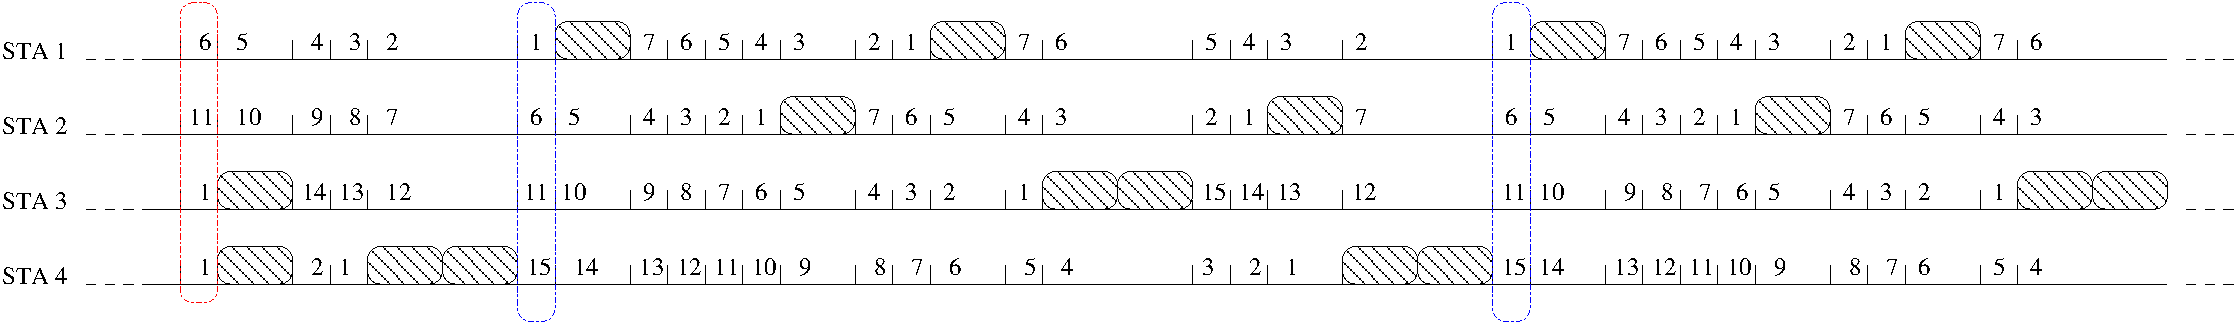
\includegraphics[width=\linewidth]{csma_eca_different_backoff-eps-converted-to.pdf}}
	\else
		(0,0) node{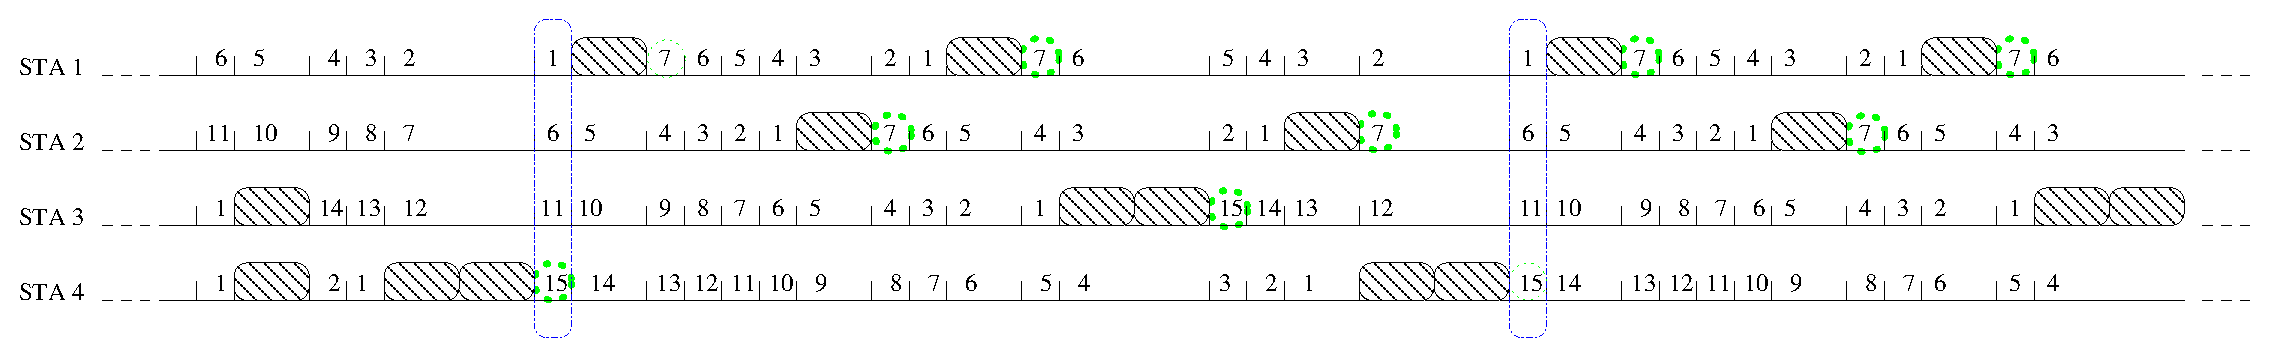
\includegraphics[width=\linewidth]{csma_eca_different_backoff.eps}}
	\fi
	(0,-1.0) node {\smaller Example balls and bins figure.};
\end{tikzpicture}
\end{center}
}

\headerbox{Ensuring fairness}{name=hysteresis,column=0,below=contention}{

This section introduces the hysteresis and fair share concepts.

\begin{center}
\begin{tikzpicture}
\path
	\ifpdf
		(0,0) node{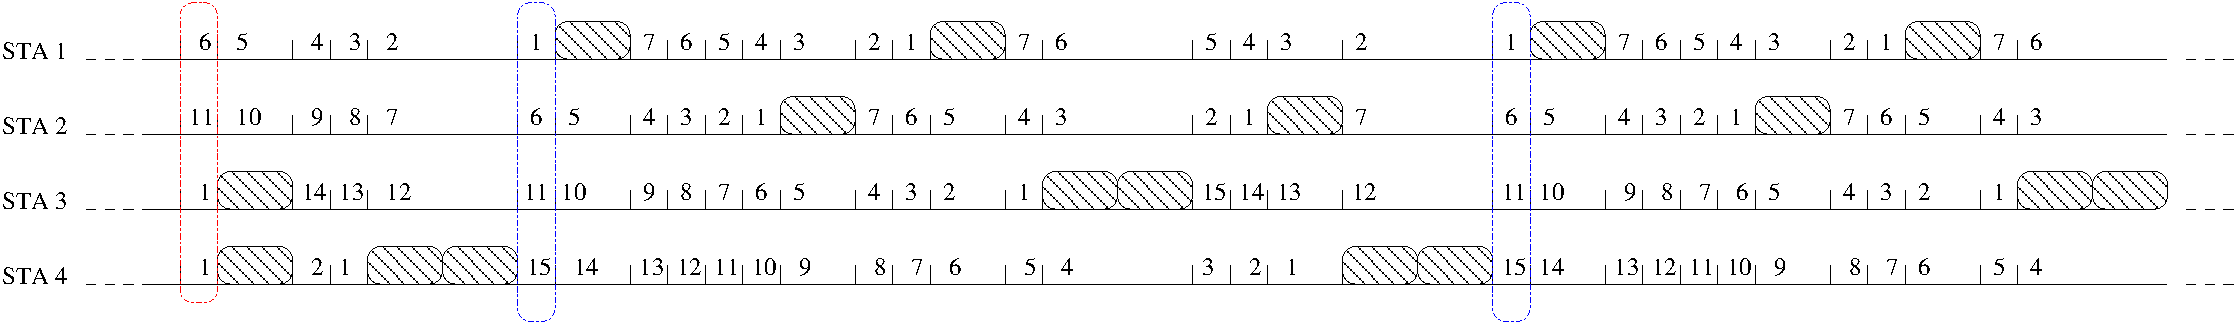
\includegraphics[width=\linewidth]{csma_eca_different_backoff-eps-converted-to.pdf}}
	\else
		(0,0) node{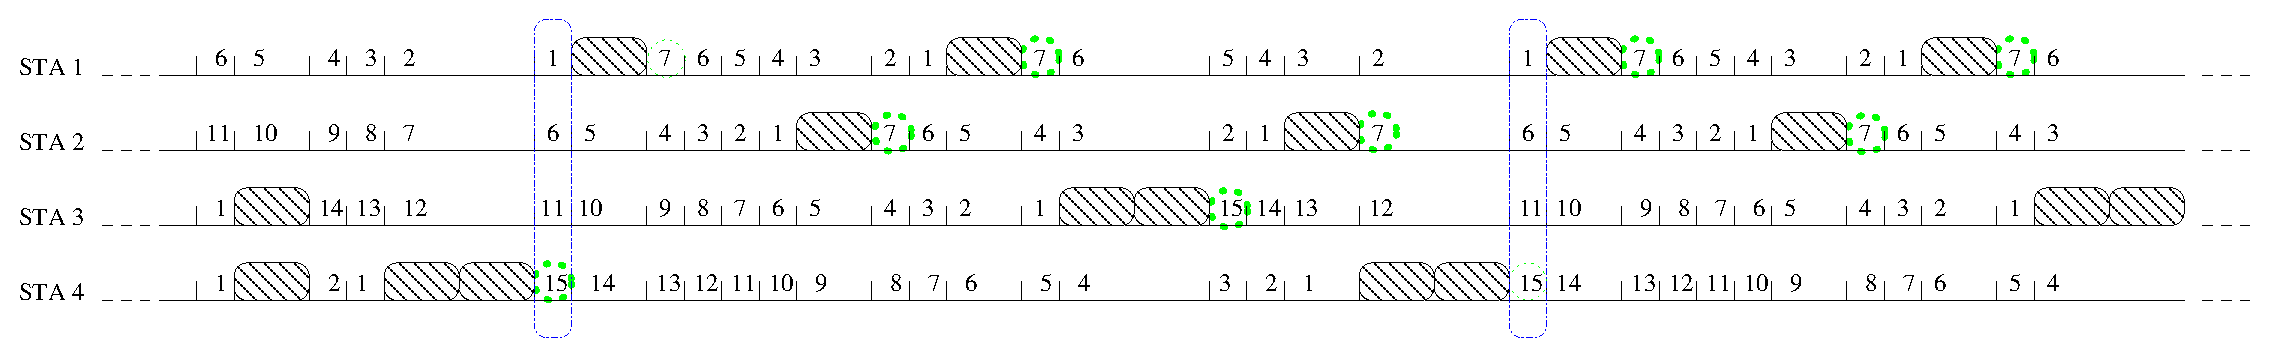
\includegraphics[width=\linewidth]{csma_eca_different_backoff.eps}}
	\fi
	(0,-1.0) node {\smaller Example balls and bins figure.};
\end{tikzpicture}
\end{center}
}

\headerbox{Throughput and fairness in CSMA/CA and CSMA/ECA}{name=throughputBasicECA,column=0,below=hysteresis,above=bottom}{

Test
\begin{center}
\begin{tikzpicture}
\path
	\ifpdf
		(0,0) node{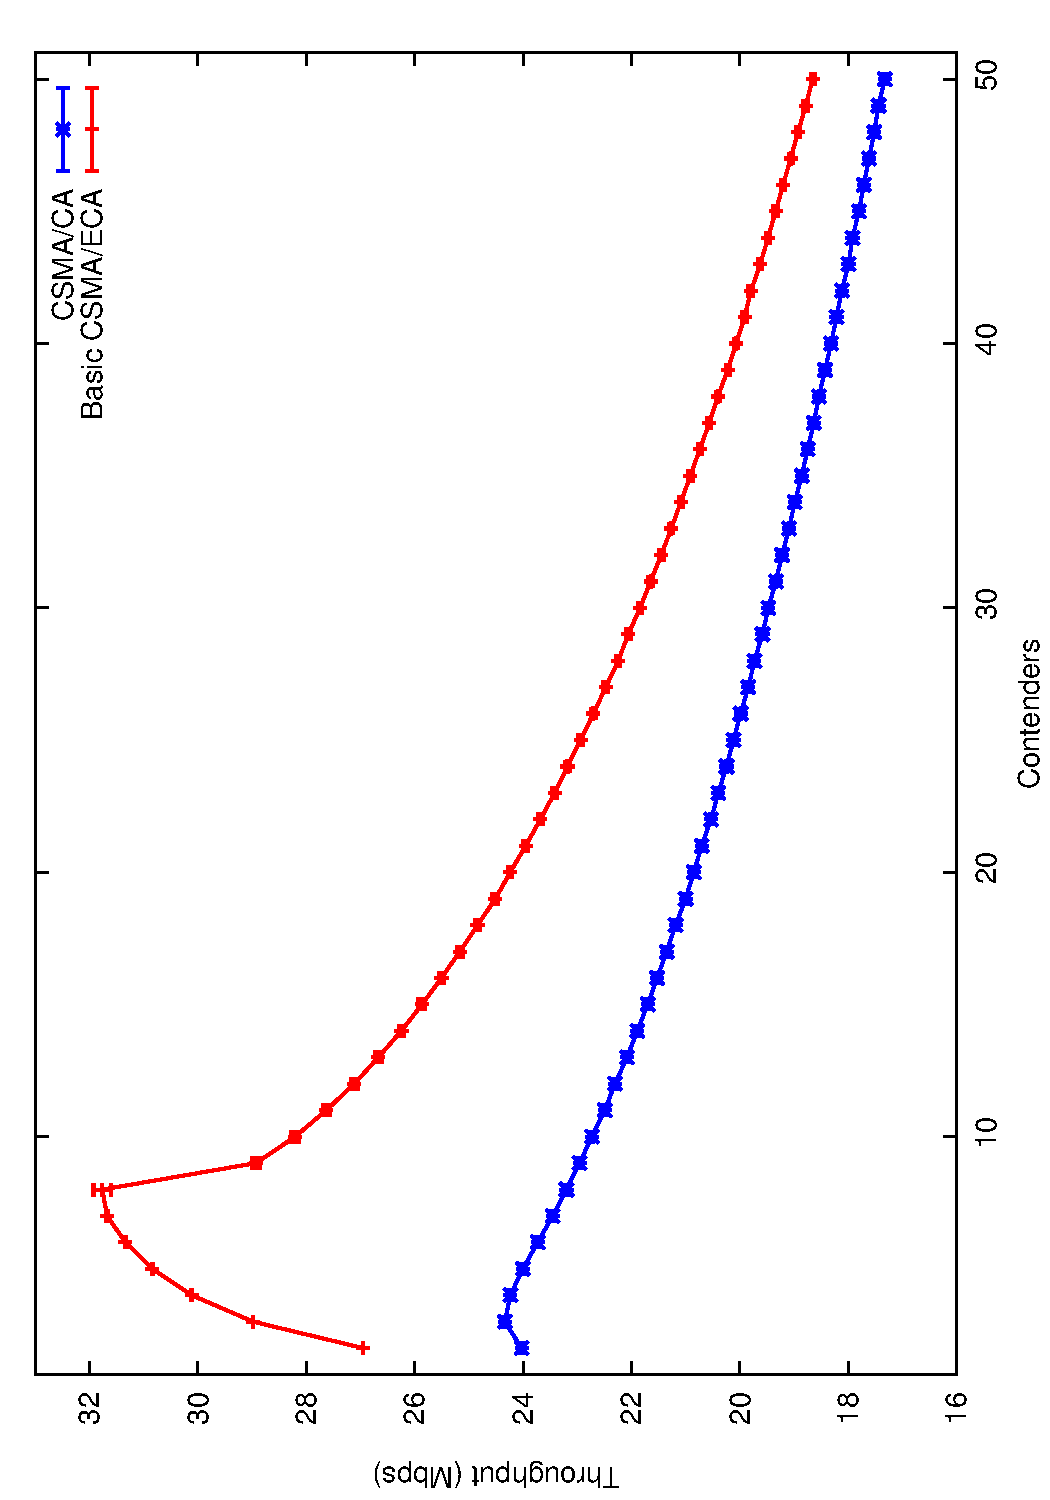
\includegraphics[width=0.7\linewidth, angle=-90]{DCF-ECA-eps-converted-to.pdf}}
	\else
		(0,0) node{\includegraphics[width=\linewidth]{DCF-ECA.eps}}
	\fi
	(0,-4.2) node {\smaller Example balls and bins figure.};
\end{tikzpicture}
\end{center}

}

\headerbox{CSMA/ECA: hysteresis and fair share}{name=fullECA,column=1,span=1,below=motivation}{

Explanation on how the hysteresis and fair share achieve this increase in throughput. Also to mention the resiliency to slot drift.

\begin{center}
\begin{tikzpicture}
\path
	\ifpdf
		(0,0) node{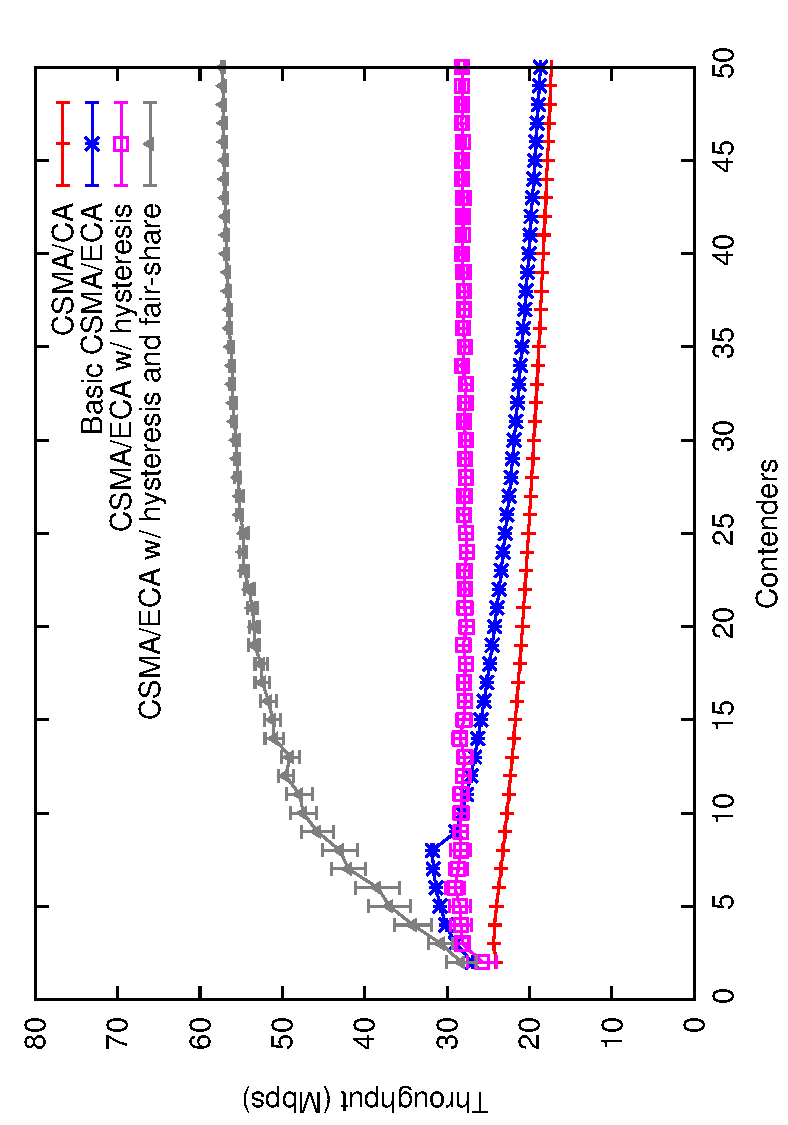
\includegraphics[width=0.7\linewidth, angle=-90]{throughput-combined-eps-converted-to.pdf}}
	\else
		(0,0) node{\includegraphics[width=0.7\linewidth]{throughput-combined.eps}}
	\fi
	(0,-4.2) node {\smaller An STB establishes active (used) and inactive (unused) SIP sessions.};
\end{tikzpicture}
\end{center}

}

\headerbox{Future plans}{name=future,column=1,below=fullECA,above=references}{

Some of the future directions of the project:
\begin{itemize}
	\item Unsaturated scenarios.
	\item To implement IEEE 802.11e EDCA.
	\item Wireless MAC Processors.
	\item Implementation in RFID networks.
\end{itemize}

\begin{center}
\begin{tikzpicture}
\path
	\ifpdf
		(0,0) node{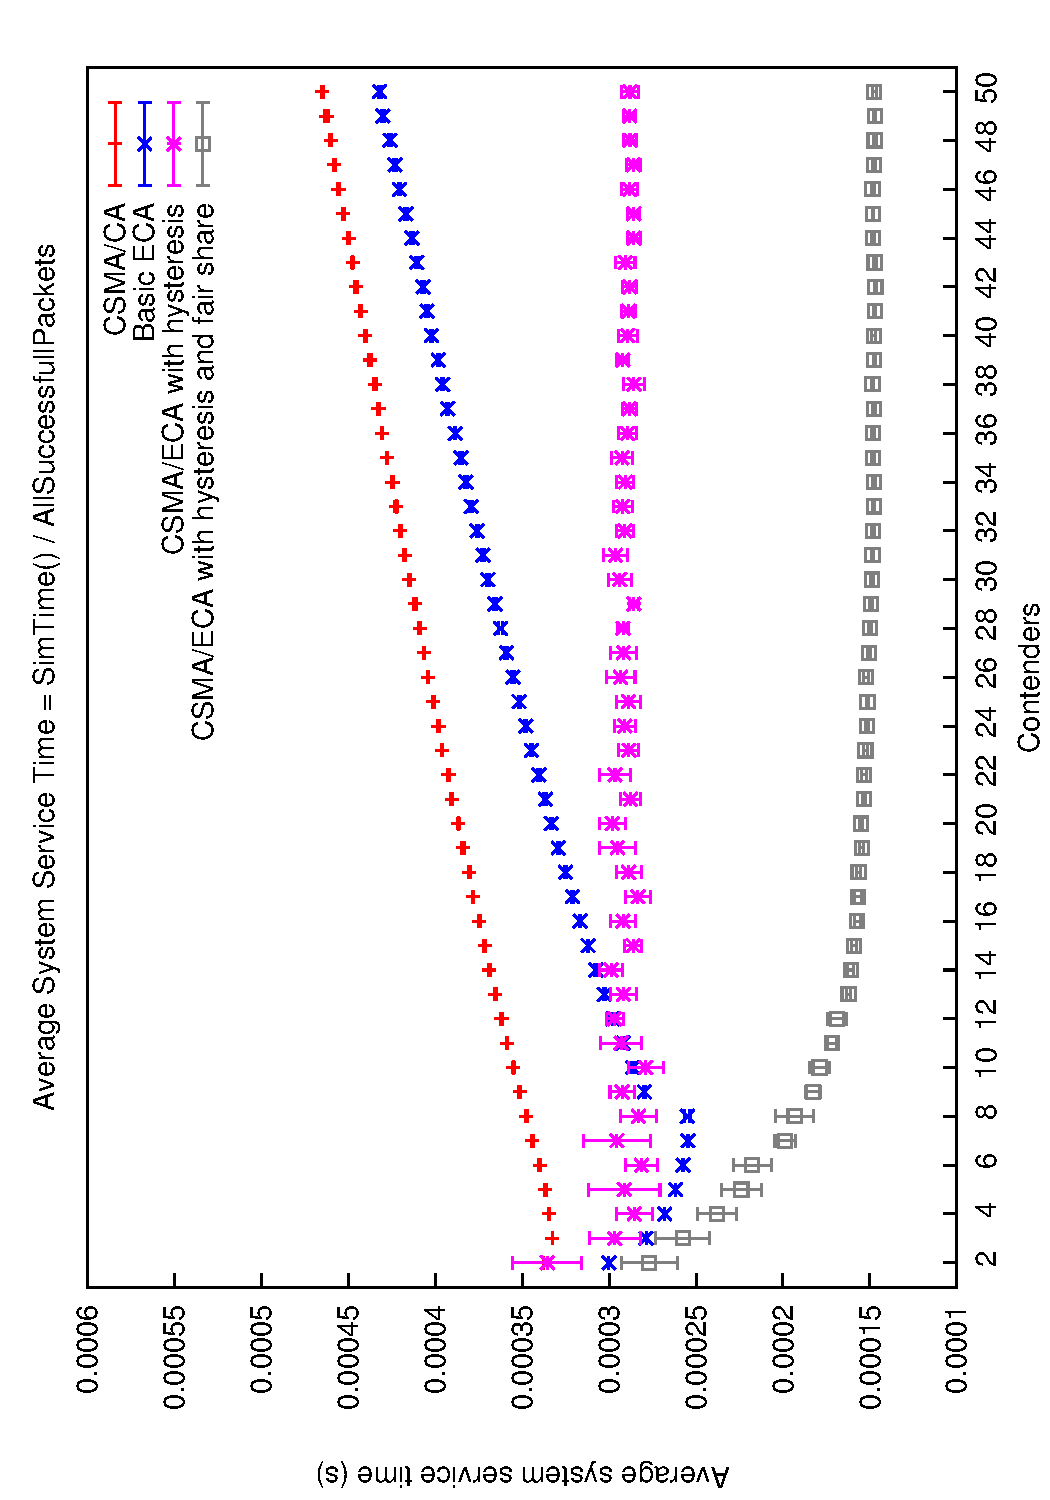
\includegraphics[width=0.5\linewidth, angle=-90]{avgSystemServiceTime-eps-converted-to.pdf}}
	\else
		(0,0) node{\includegraphics[width=0.5\linewidth]{avgSystemServiceTime.eps}}
	\fi
	(0,-3.2) node {\smaller Average system service time.};
\end{tikzpicture}
\end{center}

}

\headerbox{References}{name=references,span=1,column=1,above=bottom}{

{
\scriptsize

\renewcommand*{\refname}{\vspace*{-0.5em}}
\let\oldbibliography\thebibliography
\renewcommand{\thebibliography}[1]{\oldbibliography{#1}\setlength{\itemsep}{-0.3em}}

\begin{thebibliography}{1}

\bibitem{bikfalvi2009ijcs}
Alex Bikfalvi, Jaime Garc\'{i}a-Reinoso, Iv\'{a}n Vidal, and Francisco Valera.
\newblock A peer-to-peer iptv service architecture for the ip multimedia
  subsystem.
\newblock {\em International Journal of Communication Systems},
  23(6--7):780--801, June--July 2009.

\bibitem{qiu2009modelinguser}
T.~Qiu, Z.~Ge, S.~Lee, J.~Wang, J.~Xu, and Q.~Zhao.
\newblock Modeling user activities in a large iptv system.
\newblock In {\em Proceedings of the 9th ACM SIGCOMM conference on Internet
  measurement conference}, pages 430--441. ACM, 2009.

\bibitem{qiu2009modelingchannel}
T.~Qiu, Z.~Ge, S.~Lee, J.~Wang, Q.~Zhao, and J.~Xu.
\newblock Modeling channel popularity dynamics in a large iptv system.
\newblock In {\em Proceedings of the eleventh international joint conference on
  Measurement and modeling of computer systems}, pages 275--286. ACM, 2009.

\end{thebibliography}
}

}

\end{poster}

\end{document}
